\documentclass[11pt,a4paper]{article}
\usepackage{amsmath}
\usepackage{enumerate}
\usepackage{fancyhdr}
\usepackage{graphicx}
\usepackage[utf8]{inputenc}
\usepackage[a4paper, top=1in, bottom=1.25in, left=0.75in, right=0.75in]{geometry}

\begin{document}
\pagestyle{fancy}
\fancyhead[R]{Niels Hoppe xxxxxx, Robert Schüle xxxxxx, Christoph Ende 331655}

\section{Connectionist Neurons and Multi Layer Perceptrons}

%%%%%%%%%%%%%%%%%%%%%%%%%%%%%%%%%%%%%%%%%%%%%%%%%%%%%%%%%%%%%%%%%%%%%%%%%%%%%%%%
\subsection{Terminology}

\begin{enumerate}[a)]
\item

As 3-layered networks with linear transfer functions are equivalent to a single connectionist neuron (p.13), non-linear transfer functions are required achieve the computational capabilities to approximate more complex functions or model more complex behaviour. Basically, we end up with only linear decision boundaries, which might not be sufficient to seperate our data points effectively.

\item

The bias serves as a threshold for the activity signal (p.12). Modifying the threshold moves the decision boundary while preserving it's slope.

In figure 8 of the script (p.8) we see a working example with a bias. If we didn't have a bias, the decision boundary would pass through the origin, making it impossible to reliably distinguish apple-datapoints from orange-datapoints, regardless of it's slope.

\item

Point and edge filters (Sobel filters) are specific linear weights ($w$) for the input vector $x$, used for point and edge detection in images.

\item

The stochastic function has a negative slope at the inflection point and is not deterministic.

\end{enumerate}
%%%%%%%%%%%%%%%%%%%%%%%%%%%%%%%%%%%%%%%%%%%%%%%%%%%%%%%%%%%%%%%%%%%%%%%%%%%%%%%%
\subsection{Finding Parameters of a Connectionist Neuron}

\begin{enumerate}[a)]
\item


\end{enumerate}
%%%%%%%%%%%%%%%%%%%%%%%%%%%%%%%%%%%%%%%%%%%%%%%%%%%%%%%%%%%%%%%%%%%%%%%%%%%%%%%%
\subsection{Learning paradigms}

\begin{enumerate}[a)]
\item

\item
\begin{figure}[h]
  \centering
  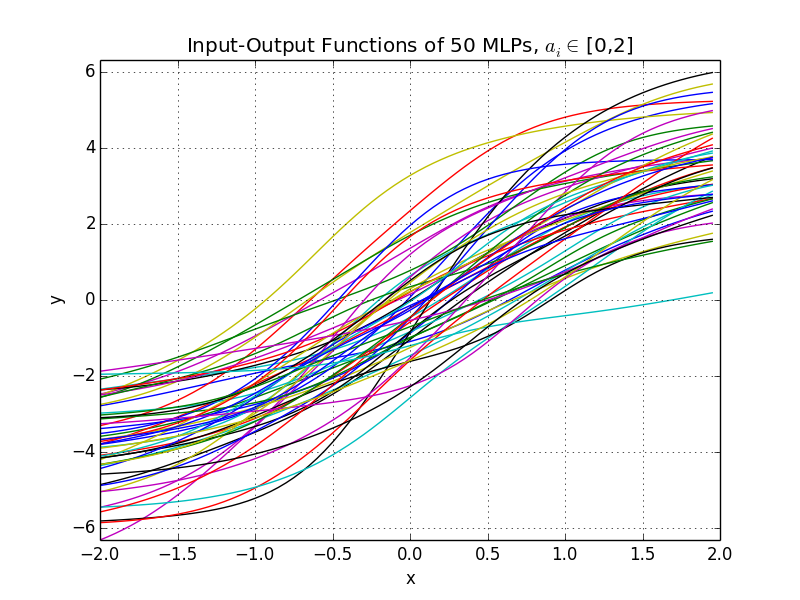
\includegraphics[width=13 cm]{23b.png}
  %\caption{Energy Decay Curve}
  \label{23b}
\end{figure}


\item
\begin{figure}[h]
  \centering
  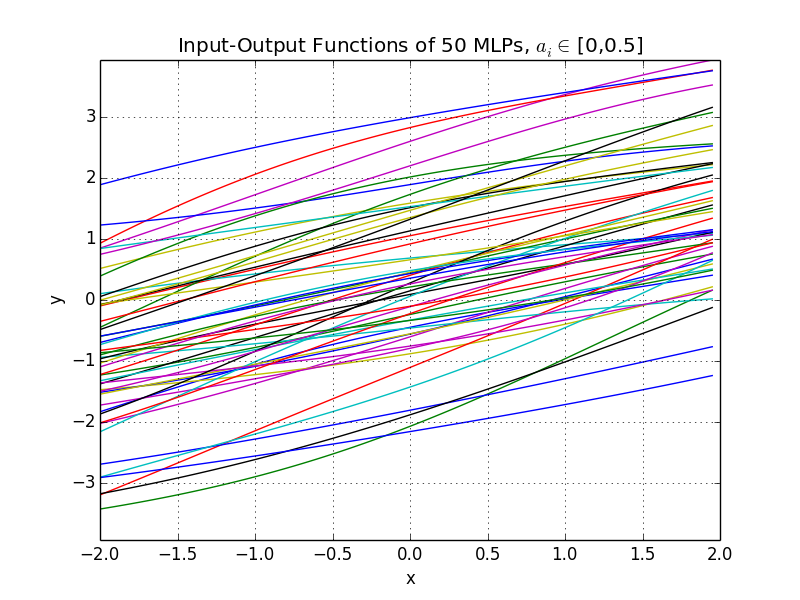
\includegraphics[width=13 cm]{23c.png}
  %\caption{Energy Decay Curve}
  \label{23c}
\end{figure}


\end{enumerate}
%%%%%%%%%%%%%%%%%%%%%%%%%%%%%%%%%%%%%%%%%%%%%%%%%%%%%%%%%%%%%%%%%%%%%%%%%%%%%%%%
\end{document}
